Аукцион это популярный публчиный инструмент реализации имущества с ценнобразованием.


\textit{Определение} В \textbf{аукционе} участвует $n$ агентов, предоставляющий набор лотов. 
Для простоты рассмотрим случай одного товара $x$. 
Тогда введем \textit{внутреннюю} монетарную оценку $u_i$ товара, отражающую утилитарное восприятие агента от обладания параметра. Уточним, что мера $u_i$ является скрытой для других участников и организатора аукциона.


\begin{figure}[h]
    \centering
    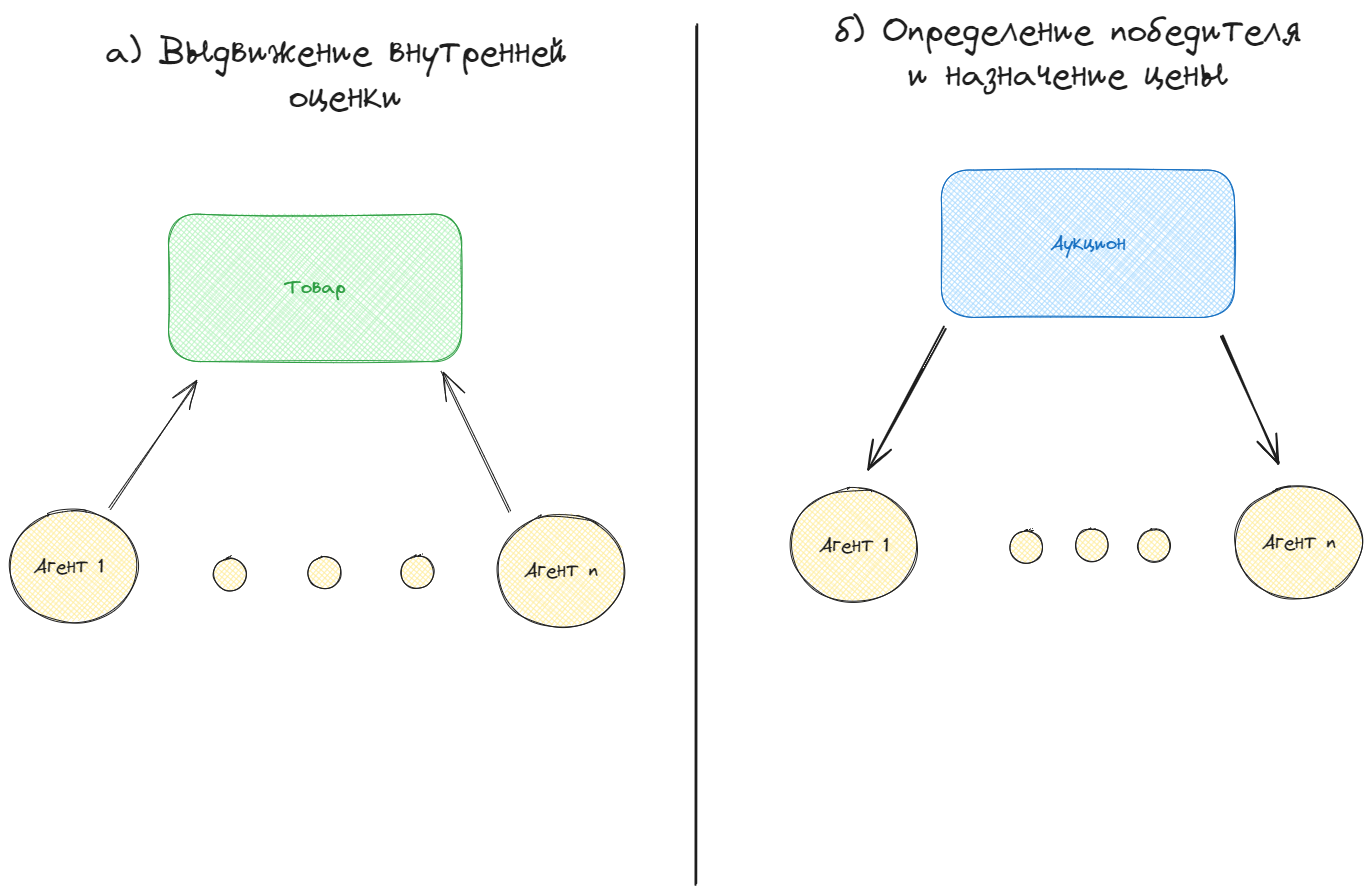
\includegraphics[width=0.5\textwidth]{assets/auctions/setting.excalidraw.png}
    \caption{Аукцион}
\end{figure}



В случае \texit{проигрыша} в аукционе агент


Аукцион определяет победителя аукциона